% Coulomb (dry) friction added to the dual-gantry LPV-LFR baseline.
% Self-contained: shows the baseline (the model we augment) and the single-
% substitution friction addition. Notation follows Hoekstra et al. (2025) and
% matches docs/writeup/jan-augmentation-writeup.tex. Compile: pdflatex.
\documentclass[11pt]{article}

\usepackage[a4paper,margin=2.2cm]{geometry}
\usepackage[T1]{fontenc}
\usepackage[utf8]{inputenc}
\usepackage{lmodern}
\usepackage{amsmath,amssymb,mathtools,bm}
\usepackage{microtype}
\usepackage{enumitem}
\usepackage{titlesec}
\usepackage{graphicx}
\usepackage{tikz}
\usetikzlibrary{arrows.meta,positioning,calc}
\usepackage[hidelinks]{hyperref}

\titleformat{\section}{\Large\bfseries}{\thesection}{0.75em}{}
\titleformat{\subsection}{\large\bfseries}{\thesubsection}{0.75em}{}
\titlespacing*{\section}{0pt}{1.4ex plus .2ex minus .2ex}{0.9ex}
\titlespacing*{\subsection}{0pt}{1.0ex plus .2ex minus .2ex}{0.5ex}

\newcommand{\R}{\mathbb{R}}
\newcommand{\adj}{\operatorname{adj}}
\newcommand{\diag}{\operatorname{diag}}
\newcommand{\sgn}{\operatorname{sign}}

\newcommand{\xb}{\tilde{x}}
\newcommand{\yh}{\hat{y}}
\newcommand{\Cbar}{\bar{C}_d}
\newcommand{\fb}{f_{\mathrm{base}}}
\newcommand{\hb}{h_{\mathrm{base}}}
\newcommand{\fc}{f_{\mathrm{c}}}
\newcommand{\ueff}{u_{\mathrm{eff}}}
\newcommand{\Fcs}{F_c^{\mathrm{s}}}

\setlist{nosep, leftmargin=1.4em}

\begin{document}

\begin{center}
  {\LARGE\bfseries Adding Coulomb (dry) friction to the LPV--LFR baseline}\\[0.4em]
  {\large Dirk van den Berg}\\[0.2em]
  {\small Notation follows Hoekstra et al.\ (2025); the friction enters as a single
   substitution on the input of the baseline model.}
\end{center}
\vspace{0.4em}

% ======================================================================
\section{Baseline: the model we augment \quad (Eq.~2)}
% ======================================================================

\noindent\textbf{Coordinates and state.}
\begin{equation}
  q = [\,X,\Theta,Y\,]^\top , \qquad
  \xb = [\,X,\Theta,Y,\dot X,\dot\Theta,\dot Y\,]^\top \in \R^6 ,
  \label{eq:baseline-state}
\end{equation}
with $\xb$ the state of the three degree-of-freedom rigid gantry and $Y$ the scheduling
variable.

\medskip\noindent\textbf{Equations of motion.}
\begin{equation}
  M(Y)\,\ddot q + C\,\dot q + K\,q = P^\top u ,
  \label{eq:baseline-eom}
\end{equation}
with $u = [\,F_1,F_2,F_y\,]^\top \in \R^3$ the stage forces and $P$ the force map
(Eq.~\ref{eq:baseline-out}).

\medskip\noindent\textbf{Inertia matrix.}
\begin{equation}
  M(Y) =
  \begin{bmatrix}
    \alpha            & \beta - m_h Y      & 0 \\[2mm]
    \beta - m_h Y     & \gamma + m_h Y^2   & -m_h d \\[2mm]
    0                 & -m_h d             & m_h
  \end{bmatrix},
  \label{eq:baseline-M}
\end{equation}
with the constants
\begin{equation}
  \alpha := m_1{+}m_2{+}m_b{+}m_h , \qquad
  \beta  := \tfrac{(m_1-m_2)L_b}{2} , \qquad
  \gamma := J_b{+}J_h{+}\tfrac{(m_1+m_2)L_b^2}{4}{+}m_h d^2 .
  \label{eq:baseline-consts}
\end{equation}

\medskip\noindent\textbf{Damping and stiffness.}
\begin{equation}
  C =
  \begin{bmatrix}
    c_{g1}{+}c_{g2}             & (c_{g1}{-}c_{g2})\tfrac{L_b}{2}                    & 0 \\[2mm]
    (c_{g1}{-}c_{g2})\tfrac{L_b}{2} & c_{b1}{+}c_{b2}{+}(c_{g1}{+}c_{g2})\tfrac{L_b^2}{4} & 0 \\[2mm]
    0                          & 0                                                  & c_y
  \end{bmatrix},
  \qquad
  K =
  \begin{bmatrix}
    0 & 0            & 0 \\[2mm]
    0 & k_{b1}{+}k_{b2} & 0 \\[2mm]
    0 & 0            & 0
  \end{bmatrix}.
  \label{eq:baseline-CK}
\end{equation}

\medskip\noindent\textbf{Assumption A.}\quad
$M(Y)$ is nonsingular over the operating range, so $M(Y)^{-1}$ exists (positive-definite
inertia for all physically admissible parameters).

\medskip\noindent\textbf{Discrete-time form.}
\begin{equation}
  \xb_{k+1} = \fb(\xb_k, u_k)\ \ (\text{Eq.\ 2a}) , \qquad
  \yh_k = \hb(\xb_k, u_k) = \Cbar\,\xb_k + D_d\,u_k\ \ (\text{Eq.\ 2b}) ,
  \label{eq:baseline-io}
\end{equation}
with $\yh = [\,X_1,X_2,Y\,]^\top$ the stage positions, obtained by RK4 discretization; the
output selects positions through
\begin{equation}
  C_d = \big[\, P^\top \ \big|\ 0_{3\times3} \,\big] , \qquad
  P =
  \begin{bmatrix}
    1 & 1 & 0 \\
    \tfrac{L_b}{2} & -\tfrac{L_b}{2} & 0 \\
    0 & 0 & 1
  \end{bmatrix} , \qquad
  D_d = 0 ,
  \label{eq:baseline-out}
\end{equation}
and $\Cbar$ is $C_d$ after input/output normalization.

% ======================================================================
\section{Augmentation, part~I: Coulomb (dry) friction \quad (Eq.~3)}
% ======================================================================

\noindent\textbf{Structure.}\quad
Each of the three actuators exhibits dry friction opposing its own motion. This is a
generalized force that enters the model exactly like the stage force $u$: through the
force map $P^\top$ of Eq.~\eqref{eq:baseline-eom}. The whole addition is therefore a single
substitution on the input, and the baseline realization is reused unchanged.

\medskip\noindent\textbf{Coulomb stage force.}\quad
In the stage (per-actuator) frame the friction is diagonal,
\begin{equation}
  \Fcs(\dot q) \;=\; c_c \odot \sigma\!\big(P^\top \dot q\big),
  \qquad c_c = [\,c_{c1},\,c_{c2},\,c_{cy}\,]^\top \ge 0,
  \label{eq:coulomb-stage}
\end{equation}
where $P^\top \dot q \in \R^3$ are the stage velocities (the derivatives of the measured
stage positions of Eq.~\eqref{eq:baseline-out}), $\odot$ is the elementwise (Hadamard)
product, $c_c$ collects the per-actuator Coulomb magnitudes, and $\sigma$ is applied
componentwise:
\begin{equation}
  \sigma(v) = \tanh\!\big(v/v_0\big)\quad\text{(smooth, for gradient-based training)}
  \qquad\text{or}\qquad
  \sigma(v) = \sgn(v)\quad\text{(ideal)} .
  \label{eq:coulomb-sigma}
\end{equation}
The transition width $v_0>0$ is a hyperparameter (heuristic); $\sigma \to \sgn$ as
$v_0 \to 0$. The smooth form is used for backpropagation through time (Makkar \& Dixon,
2005); the ideal form is a reference.

\medskip\noindent\textbf{Augmented equations of motion.}\quad
Friction opposes the applied force per actuator, i.e.\ it acts as an effective stage force
\begin{equation}
  \ueff \;=\; u - \Fcs(\dot q) \;=\; u - c_c \odot \sigma\!\big(P^\top \dot q\big),
  \label{eq:coulomb-ueff}
\end{equation}
and Eq.~\eqref{eq:baseline-eom} becomes
\begin{equation}
  \boxed{\;M(Y)\,\ddot q + C\,\dot q + K\,q
    \;=\; P^\top \ueff
    \;=\; P^\top\!\big(u - c_c \odot \sigma(P^\top \dot q)\big).\;}
  \label{eq:coulomb-eom}
\end{equation}
The inertia $M(Y)$, damping $C$, stiffness $K$, force map $P^\top$, Assumption~A, and the
output map~\eqref{eq:baseline-out} are all unchanged; only the input is redefined.
Equivalently, an explicit solve gives
\begin{equation}
  \ddot q \;=\; M(Y)^{-1}\!\big(P^\top \ueff - C\,\dot q - K\,q\big).
  \label{eq:coulomb-explicit}
\end{equation}

\medskip\noindent\textbf{Discrete-time form.}\quad
Under the same RK4 discretization, Eq.~\eqref{eq:baseline-io} becomes
\begin{equation}
  \xb_{k+1} = \fc(\xb_k, u_k), \qquad
  \fc(\xb, u) \;\equiv\; \fb\!\big(\xb,\; u - c_c \odot \sigma(P^\top \dot q)\big),
  \label{eq:coulomb-disc}
\end{equation}
i.e.\ $\fc$ is the baseline map $\fb$ evaluated at the effective input $\ueff$; the output
map $\hb$ of Eq.~\eqref{eq:baseline-io} is unchanged.

\medskip\noindent\textbf{Block-diagram view.}\quad
A single memoryless feedback nonlinearity, tapped from the velocity states and subtracted
at the input summing node; the baseline block is reused unchanged.
\begin{center}
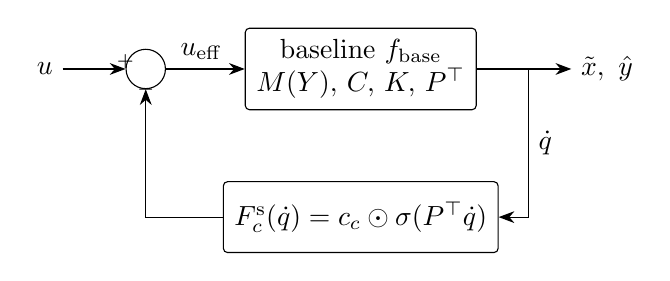
\begin{tikzpicture}[
    >={Stealth[length=2mm]},
    box/.style={draw, rounded corners=1.5pt, minimum height=9mm, inner sep=4pt, align=center},
    sum/.style={draw, circle, inner sep=0pt, minimum size=5mm},
    node distance=10mm,
  ]
  \node (in)  {$u$};
  \node[sum, right=8mm of in] (s) {};
  \node[box, right=10mm of s] (base) {baseline $\fb$\\ $M(Y),\,C,\,K,\,P^\top$};
  \node[right=12mm of base] (out) {$\xb,\ \yh$};
  \node[box, below=9mm of base] (fc) {$\Fcs(\dot q)=c_c\odot\sigma(P^\top\dot q)$};

  \draw[->] (in) -- (s);
  \draw[->] (s) -- node[above,pos=0.45]{$\ueff$} (base);
  \draw[->] (base) -- (out);
  % feedback tap of the velocity states
  \coordinate (tap) at ($(base.east)!0.55!(out.west)$);
  \draw[->] (tap) |- node[right,pos=0.25]{$\dot q$} (fc.east);
  \draw[->] (fc.west) -| (s);
  \node at ($(s)+(0,-2.6mm)$) {\scriptsize$-$};
  \node at ($(s)+(-2.6mm,0.9mm)$) {\scriptsize$+$};
\end{tikzpicture}
\end{center}

\medskip\noindent\textbf{Consistency and verification.}\quad
\begin{itemize}
  \item \emph{Reduction to baseline.} $c_c = 0 \Rightarrow \ueff = u \Rightarrow \fc \equiv \fb$;
        the augmentation vanishes exactly (verified bit-for-bit against the baseline
        forward).
  \item \emph{Realization independence.} The LFR/state-space delivery form (analytic
        $M(Y)^{-1}$ loop, unchanged $G$) reproduces the explicit solve
        Eq.~\eqref{eq:coulomb-explicit} to machine precision, including at $Y=0$.
  \item \emph{Reference EOM.} The forward matches the supervisor's direct MATLAB
        \texttt{gantrySystem}+Coulomb equations of motion to $\sim\!10^{-18}$\,m over a
        multi-thousand-step RK4 trajectory with active friction.
\end{itemize}

\medskip\noindent\textbf{Remark (state-space realization).}\quad
At the descriptor level of Eq.~\eqref{eq:coulomb-eom} the substitution
$u \mapsto \ueff$ is unambiguous. In the explicit LFR state-space realization the input
$u$ appears at more than one port (the direct input term and the scheduling path), so
$\ueff$ must replace $u$ at \emph{every} occurrence of the input; substituting at only one
port makes the friction spuriously vanish at $Y=0$. This subtlety does not arise at the
equation-of-motion level above, which is why the friction is most cleanly introduced here.

\medskip\noindent\textbf{Note on hyperparameters.}\quad
$v_0$ (transition width) is a heuristic; the small-signal slope of the smooth Coulomb term
is $c_c/v_0$, which acts as an effective near-zero-velocity damping and is not innocuous
for closed-loop behaviour. The $\tanh$-vs-$\sgn$ choice is a modeling decision, stated
explicitly rather than left implicit.

\end{document}
